\documentclass[conference]{IEEEtran}
\IEEEoverridecommandlockouts
\usepackage{cite}
\usepackage{amsmath,amssymb,amsfonts}
\usepackage{algorithmic}
\usepackage{algorithm}
\usepackage{graphicx}
\usepackage{textcomp}
\usepackage{xcolor}
\usepackage{listings}
\usepackage{tikz}
\usepackage{booktabs}
\usepackage{multirow}
\usepackage{url}
\usetikzlibrary{shapes.geometric, arrows.meta, positioning, calc}

\lstset{
  language=C,
  basicstyle=\ttfamily\footnotesize,
  keywordstyle=\color{blue}\bfseries,
  commentstyle=\color{green!50!black},
  stringstyle=\color{red},
  numbers=left,
  numberstyle=\tiny,
  breaklines=true,
  frame=single,
  captionpos=b
}

\tikzstyle{block} = [rectangle, draw, fill=blue!15, text width=5em, text centered, rounded corners, minimum height=3em]
\tikzstyle{arrow} = [thick,->,>=stealth]
\tikzstyle{decision} = [diamond, draw, fill=yellow!20, text width=4em, text centered, inner sep=0pt]
\tikzstyle{io} = [trapezium, trapezium left angle=70, trapezium right angle=110, draw, fill=green!15, text width=4em, text centered, minimum height=2.5em]

\def\BibTeX{{\rm B\kern-.05em{\sc i\kern-.025em b}\kern-.08em
    T\kern-.1667em\lower.7ex\hbox{E}\kern-.125emX}}
\begin{document}

\title{Stock Market Data Aggregator: A Multi-Module System Leveraging Advanced Data Structures for Real-Time Financial Data Processing}

\author{\IEEEauthorblockN{1\textsuperscript{st} Krushnamegh Chakke}
\IEEEauthorblockA{\textit{B.Tech CSE (AI \& ML)} \\
\textit{Vishwakarma Institute of Technology}\\
Pune, India \\
krushnamegh.chakke24@vit.edu}
\and
\IEEEauthorblockN{2\textsuperscript{nd} Sanskar Bhandari}
\IEEEauthorblockA{\textit{B.Tech CSE (AI \& ML)} \\
\textit{Vishwakarma Institute of Technology}\\
Pune, India \\
sanskarbhandari01@gmail.com}
\and
\IEEEauthorblockN{3\textsuperscript{rd} Pranav Bhandare}
\IEEEauthorblockA{\textit{B.Tech CSE (AI \& ML)} \\
\textit{Vishwakarma Institute of Technology}\\
Pune, India \\
pranavbhandare3108@gmail.com}
\and
\IEEEauthorblockN{4\textsuperscript{th} Snehal Bandgar}
\IEEEauthorblockA{\textit{B.Tech CSE (AI \& ML)} \\
\textit{Vishwakarma Institute of Technology}\\
Pune, India \\
snehal.bandgar24@vit.edu}
\and
\IEEEauthorblockN{5\textsuperscript{th} Abhishek Bhangdiya}
\IEEEauthorblockA{\textit{B.Tech CSE (AI \& ML)} \\
\textit{Vishwakarma Institute of Technology}\\
Pune, India \\
abhishebhangdiya0@gmail.com}
}

\maketitle

\begin{abstract}
Stock markets produce enormous volumes of transactional data every second, making efficient data management a critical challenge for modern financial systems. This paper presents the design and implementation of a Stock Market Data Aggregator system built entirely in C, which integrates five distinct advanced data structures to handle different aspects of real-time stock data processing. The system employs a Hash Table with chaining (using the djb2 hash function) for constant-time stock price lookups, a Priority Queue backed by a min-heap for urgency-based processing of trade alerts, an AVL Tree for maintaining sorted historical price records with guaranteed logarithmic-time operations, a dual Max/Min Heap system for dynamically ranking top-gaining and top-losing stocks, and a Trie (prefix tree) for providing fast auto-complete suggestions on stock ticker symbols. All five modules share a common data header (\texttt{stock\_data.h}) defining standardized stock record structures and sample datasets. Each module is independently implemented and tested with realistic market data simulating actual trading scenarios. We analyze the time and space complexity of each data structure, discuss collision handling, priority-based alert dispatching, self-balancing rotations, heapification procedures, and prefix-based traversal strategies. Experimental results demonstrate that the combined system achieves O(1) average-case lookups, O(log n) priority-ordered alert processing, O(log n) sorted insertions, and O(m) prefix searches, validating the suitability of advanced data structures for financial data processing applications.
\end{abstract}

\begin{IEEEkeywords}
advanced data structures, hash table, priority queue, AVL tree, heap, trie, stock market, real-time data processing
\end{IEEEkeywords}

\section{Introduction}

The global financial markets generate massive quantities of data on a continuous basis. Major stock exchanges such as the NYSE and NASDAQ collectively handle billions of data points each trading day, including price quotes, volume figures, trade timestamps, and various derived metrics \cite{b1}. Processing, storing, and querying this data in real time is a fundamental challenge for trading platforms, portfolio management systems, and market analytics tools.

Traditional approaches that rely on simple arrays or linear linked lists quickly become bottlenecks when the volume of data scales up. For instance, searching for a specific stock's current price in an unsorted array requires O(n) time, which is unacceptable when thousands of lookups need to happen every second. Similarly, maintaining sorted historical data in a plain binary search tree can degrade to O(n) in the worst case if the tree becomes skewed. Processing market alerts without priority differentiation means critical events like circuit breakers or trading halts get delayed behind routine price ticks. These performance limitations motivate the use of advanced data structures that provide better asymptotic guarantees.

In this paper, we present a modular stock market data aggregation system implemented in C that leverages five advanced data structures, each chosen to address a specific aspect of market data processing:

\begin{enumerate}
\item \textbf{Hash Table with Chaining}: Provides O(1) average-case lookup and insertion for current stock prices indexed by ticker symbol, using the djb2 hash function.
\item \textbf{Priority Queue (Min-Heap)}: Processes incoming stock alerts by urgency level---critical circuit breaker alerts are served before routine price ticks, regardless of arrival order.
\item \textbf{AVL Tree}: Stores historical price records sorted by timestamp, ensuring O(log n) search and insertion through self-balancing rotations.
\item \textbf{Max/Min Heap Pair}: Efficiently tracks top-gaining and top-losing stocks with O(1) access to the best/worst performers and O(log n) insertion.
\item \textbf{Trie (Prefix Tree)}: Enables fast auto-complete functionality for stock ticker symbols with O(m) prefix-based search, where m is the prefix length.
\end{enumerate}

All five modules are integrated through a shared header file (\texttt{stock\_data.h}) that defines common data types, sample stock records, and constants---ensuring data consistency across the entire system.

The rest of this paper is organized as follows. Section II reviews related literature. Section III states the problem. Section IV describes our methodology. Section V presents the system design. Section VI details algorithm design with pseudocode and complexity analysis. Section VII covers implementation specifics. Section VIII discusses results. Section IX outlines advantages and limitations. Section X suggests future work, and Section XI concludes the paper.

\section{Literature Review}

\subsection{Hash Tables in Financial Systems}

Hash tables are widely used in high-frequency trading systems where constant-time access to instrument data is critical. Cormen et al. \cite{b2} provide a comprehensive treatment of hash table design, covering universal hashing, open addressing, and chaining-based collision resolution. The djb2 hash function, originally proposed by Bernstein, has been shown to provide good distribution characteristics for short string keys \cite{b3}, making it suitable for stock ticker symbols which are typically 1--5 characters long.

\subsection{Priority Queues for Event-Driven Systems}

Priority queues are essential in systems where events must be processed based on urgency rather than arrival order. Cormen et al. \cite{b2} discuss binary heap-based priority queue implementations providing O(log n) insertion and extraction. In financial systems, trading halts and circuit breakers must be processed immediately, while routine price updates can tolerate delay. Sedgewick and Wayne \cite{b4} further describe min-heap-based priority queues where the smallest key (highest urgency) is always at the root, enabling O(1) peek and O(log n) extraction of the most critical alert.

\subsection{Self-Balancing Trees for Time-Series Data}

Adelson-Velsky and Landis introduced the AVL tree in 1962 as the first self-balancing binary search tree \cite{b5}. AVL trees guarantee that the height difference between left and right subtrees of any node is at most one, ensuring O(log n) operations even in the worst case. Knuth \cite{b6} further analyzed the four rotation cases (LL, RR, LR, RL) required to maintain this balance. For time-series financial data, AVL trees prevent the degenerate linear-chain behavior that would afflict a plain BST when records arrive in roughly chronological order.

\subsection{Heaps for Ranking and Extrema}

Williams \cite{b7} introduced the binary heap as an efficient implementation of the priority queue abstract data type. In stock market contexts, heaps are naturally suited to maintaining rankings of top gainers and losers, as the stock with the largest (or smallest) percentage change can always be retrieved in constant time. Our system uses both max-heap and min-heap variants simultaneously---one for gainers and one for losers.

\subsection{Tries for String-Based Retrieval}

The trie data structure, introduced by Fredkin \cite{b8}, organizes strings character-by-character in a tree, enabling prefix-based retrieval in O(m) time where m is the query length. For stock symbol search interfaces, where a user might type ``A'' and expect to see ``AAPL'', ``AMD'', ``AMZN'', and ``ADBE'', the trie is a natural choice over hash tables which require exact-match queries.

\section{Problem Statement}

Modern stock exchanges produce millions of data updates per trading session. A practical stock data management system must simultaneously address several requirements:

\begin{itemize}
\item \textbf{Fast Lookup}: Given a stock ticker symbol, retrieve its current price in constant time.
\item \textbf{Priority-Based Alert Processing}: Process critical market alerts (trading halts, circuit breakers) before routine price updates, irrespective of arrival order.
\item \textbf{Sorted Historical Storage}: Store historical price records in a balanced, sorted structure that supports efficient traversal and min/max queries.
\item \textbf{Dynamic Ranking}: Continuously maintain rankings of best-performing and worst-performing stocks as new data arrives.
\item \textbf{Prefix Search}: Allow users to search for stock symbols by typing partial prefixes, with instant suggestions.
\end{itemize}

No single data structure can efficiently satisfy all these requirements simultaneously. This motivates a multi-structure architecture where each component is optimized for its specific role in the data pipeline.

\section{Methodology}

\subsection{Development Approach}

The project follows a modular design methodology with five independent C modules sharing a common header:

\begin{enumerate}
\item \textbf{Shared Header Design}: A centralized \texttt{stock\_data.h} file defines the \texttt{StockRecord} structure (containing symbol, price, volume, and change\_percent fields), the \texttt{MAX\_SYMBOL\_LEN} constant, and a \texttt{SAMPLE\_STOCKS[]} array used across all modules for consistent test data.
\item \textbf{Independent Module Development}: Each module is implemented as a separate \texttt{.c} file with its own \texttt{run\_*()} entry function, enabling isolated compilation and testing.
\item \textbf{Realistic Test Data}: All modules use actual stock ticker symbols (AAPL, GOOGL, MSFT, NVDA, etc.) with realistic price ranges and trading volumes.
\item \textbf{Build Automation}: A \texttt{Makefile} with \texttt{gcc -Wall -g} flags automates compilation of all five modules.
\end{enumerate}

\subsection{Design Principles}

\begin{itemize}
\item \textbf{Correctness First}: Each data structure maintains its structural invariants (hash table chaining, AVL balance property, heap ordering, priority queue urgency ordering) at all times.
\item \textbf{Observable Behavior}: All modules produce detailed console output showing internal operations for educational and debugging purposes.
\item \textbf{Performance Tracking}: Each module includes built-in statistics collection (collision counts, rotation counts, queue utilization).
\item \textbf{Edge Case Handling}: Boundary conditions such as full queues, empty heaps, missing search keys, and duplicate timestamp insertions are explicitly handled.
\end{itemize}

\section{System Design}

The system follows a pipeline architecture where stock market data flows through multiple processing stages. Fig.~\ref{fig:arch} illustrates the overall system architecture.

\begin{figure}[htbp]
\centering
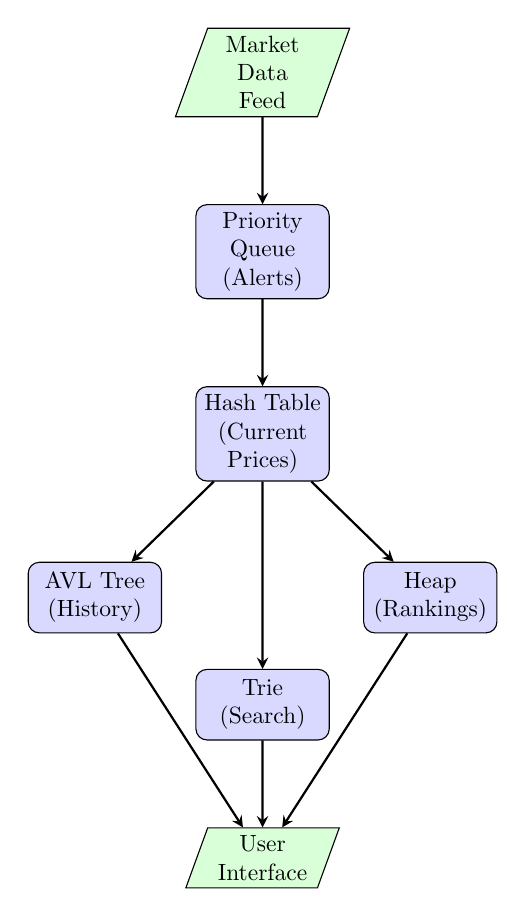
\begin{tikzpicture}[node distance=1.3cm, auto, scale=0.85, transform shape]
  \node[io] (input) {Market Data Feed};
  \node[block, below=of input] (pq) {Priority Queue (Alerts)};
  \node[block, below=of pq] (hash) {Hash Table (Current Prices)};
  \node[block, below left=1.2cm and 0.5cm of hash] (avl) {AVL Tree (History)};
  \node[block, below right=1.2cm and 0.5cm of hash] (heap) {Heap (Rankings)};
  \node[block, below=2.8cm of hash] (trie) {Trie (Search)};
  \node[io, below=of trie] (output) {User Interface};
  \draw[arrow] (input) -- (pq);
  \draw[arrow] (pq) -- (hash);
  \draw[arrow] (hash) -- (avl);
  \draw[arrow] (hash) -- (heap);
  \draw[arrow] (hash) -- (trie);
  \draw[arrow] (avl) -- (output);
  \draw[arrow] (heap) -- (output);
  \draw[arrow] (trie) -- (output);
\end{tikzpicture}
\caption{System architecture of the Stock Market Data Aggregator showing data flow from market feed through each processing module.}
\label{fig:arch}
\end{figure}

\subsection{Data Flow}

\begin{enumerate}
\item \textbf{Alert Ingestion}: Raw market events enter the Priority Queue, tagged with urgency levels (1=CRITICAL through 4=LOW).
\item \textbf{Priority Dispatch}: The Priority Queue extracts alerts by urgency---circuit breakers and trading halts (priority 1) are processed before routine price ticks (priority 4), regardless of arrival order.
\item \textbf{Price Storage}: The Hash Table stores current price for each stock symbol via the djb2 hash function, enabling O(1) lookups.
\item \textbf{Historical Logging}: Price updates are inserted into the AVL Tree indexed by timestamp for chronological analysis.
\item \textbf{Ranking Update}: Price change percentages are fed into the Max Heap (gainers) and Min Heap (losers).
\item \textbf{Symbol Indexing}: Stock symbols are indexed in the Trie for auto-complete queries.
\end{enumerate}

\subsection{Module Interfaces}

Table~\ref{tab:interfaces} summarizes the primary operations of each module.

\begin{table}[htbp]
\caption{Module Interfaces and Primary Operations}
\begin{center}
\begin{tabular}{|l|l|l|}
\hline
\textbf{Module} & \textbf{Key Operations} & \textbf{Complexity} \\
\hline
Hash Table & ht\_insert, ht\_search & O(1) avg \\
\hline
Priority Queue & pq\_insert, pq\_extract & O(log n) \\
\hline
AVL Tree & avl\_insert, inorder & O(log n) \\
\hline
Heap & heap\_insert, heap\_extract & O(log n) / O(1) \\
\hline
Trie & trie\_insert, get\_suggestions & O(m) \\
\hline
\end{tabular}
\label{tab:interfaces}
\end{center}
\end{table}

\section{Algorithm Design}

\subsection{Hash Table -- djb2 Hashing with Chaining}

The hash table uses the djb2 algorithm to map stock ticker strings to bucket indices. The function computes $h = ((h \ll 5) + h) + c$ iteratively for each character $c$, starting from $h = 5381$, then takes the result modulo the table size (100).

\begin{algorithm}
\caption{Hash Table Insert/Update (\texttt{ht\_insert})}
\begin{algorithmic}[1]
\REQUIRE Hash table $HT$, symbol $s$, price $p$, volume $v$
\STATE $idx \gets \text{hash}(s) \mod \text{TABLE\_SIZE}$
\STATE $cur \gets HT.buckets[idx]$
\WHILE{$cur \neq \text{NULL}$}
  \IF{$cur.symbol = s$}
    \STATE $cur.change \gets ((p - cur.price)/cur.price) \times 100$
    \STATE $cur.price \gets p$; $cur.volume \gets v$
    \RETURN \COMMENT{Update existing entry}
  \ENDIF
  \STATE $cur \gets cur.next$
\ENDWHILE
\STATE Create new node $n$ with $(s, p, v)$
\STATE $n.next \gets HT.buckets[idx]$ \COMMENT{Prepend to chain}
\STATE $HT.buckets[idx] \gets n$
\end{algorithmic}
\end{algorithm}

\textbf{Complexity}: Average-case O(1) for both insert and search, assuming a good hash function and load factor below 0.7. Worst-case O(n) when all keys collide into a single bucket. \textbf{Space}: O(n + TABLE\_SIZE).

\subsection{Priority Queue -- Min-Heap Based Alert Dispatch}

Unlike a simple FIFO queue, the Priority Queue uses a min-heap ordered on a 4-level urgency field (1=CRITICAL, 2=HIGH, 3=MEDIUM, 4=LOW). Each \texttt{StockAlert} contains the symbol, price, volume, priority, alert type (e.g., ``Trading HALT issued'', ``Circuit breaker -7\%''), and a timestamp. The min-heap ensures that the alert with the \emph{lowest} priority number (i.e., highest urgency) is always at the root.

\begin{algorithm}
\caption{Priority Queue Insert (\texttt{pq\_insert})}
\begin{algorithmic}[1]
\REQUIRE Priority Queue $PQ$, alert data $a$
\IF{$PQ.size = \text{PQ\_CAPACITY}$}
  \STATE Print warning; \RETURN \COMMENT{Queue full}
\ENDIF
\STATE $PQ.data[PQ.size] \gets a$
\STATE $PQ.size \gets PQ.size + 1$
\STATE heapify\_up($PQ$, $PQ.size - 1$)
\end{algorithmic}
\end{algorithm}

\begin{algorithm}
\caption{Priority Queue Extract (\texttt{pq\_extract})}
\begin{algorithmic}[1]
\REQUIRE Priority Queue $PQ$
\IF{$PQ.size = 0$}
  \RETURN empty\_error
\ENDIF
\STATE $top \gets PQ.data[0]$ \COMMENT{Highest-urgency alert}
\STATE $PQ.data[0] \gets PQ.data[PQ.size - 1]$
\STATE $PQ.size \gets PQ.size - 1$
\IF{$PQ.size > 0$}
  \STATE heapify\_down($PQ$, $0$)
\ENDIF
\RETURN $top$
\end{algorithmic}
\end{algorithm}

\textbf{Complexity}: O(log n) for both insert (heapify-up) and extract (heapify-down). O(1) peek at the highest-urgency alert. \textbf{Space}: O(PQ\_CAPACITY), fixed allocation of 100 slots.

\subsection{AVL Tree -- Self-Balancing Insertion}

The AVL tree maintains the balance invariant $|height(left) - height(right)| \leq 1$ for every node. After each insertion, the algorithm checks the balance factor and performs the appropriate rotation.

\begin{algorithm}
\caption{AVL Tree Insertion (\texttt{avl\_insert})}
\begin{algorithmic}[1]
\REQUIRE Node $root$, timestamp $ts$, price $p$, volume $v$
\IF{$root = \text{NULL}$}
  \RETURN avl\_new\_node($ts, p, v$)
\ENDIF
\IF{$ts < root.ts$}
  \STATE $root.left \gets \text{avl\_insert}(root.left, ts, p, v)$
\ELSIF{$ts > root.ts$}
  \STATE $root.right \gets \text{avl\_insert}(root.right, ts, p, v)$
\ELSE
  \STATE Update price and volume in-place; \RETURN $root$
\ENDIF
\STATE Update $root.height$
\STATE $bal \gets avl\_balance(root)$
\STATE Apply LL, RR, LR, or RL rotation if $|bal| > 1$
\RETURN $root$
\end{algorithmic}
\end{algorithm}

The four rotation cases are: LL ($bal>1$, $ts < left.ts$), RR ($bal<-1$, $ts > right.ts$), LR ($bal>1$, $ts > left.ts$), and RL ($bal<-1$, $ts < right.ts$). Each rotation involves reassigning at most two pointers and updating two heights.

\textbf{Complexity}: O(log n) for insertion and search. Tree height bounded by $1.44 \log_2(n+2)$. \textbf{Space}: O(n).

\subsection{Heap -- Dual Max/Min for Gainers and Losers}

The system creates two separate heaps from the shared \texttt{SAMPLE\_STOCKS[]} data: a Max Heap for stocks with positive \texttt{change\_percent} (gainers) and a Min Heap for stocks with negative \texttt{change\_percent} (losers). Both use array-based storage with parent at $\lfloor(i-1)/2\rfloor$ and children at $2i+1$, $2i+2$.

The \texttt{display\_top\_n} function creates a temporary copy of the heap to perform non-destructive extraction, preserving the original heap state.

\textbf{Complexity}: O(log n) insert via heapify-up, O(1) peek at top, O(log n) extract via heapify-down. \textbf{Space}: O(MAX\_HEAP\_SIZE).

\subsection{Trie -- Prefix-Based Auto-Complete}

The Trie stores stock symbols character by character. Each \texttt{TrieNode} has 26 child pointers (one per uppercase letter), an \texttt{is\_end} flag, the complete symbol string, and the last known price. The \texttt{char\_idx} function maps characters via \texttt{toupper(c) - `A'}. Node allocation uses \texttt{calloc} to zero-initialize all child pointers.

\begin{algorithm}
\caption{Trie Auto-Complete (\texttt{get\_suggestions})}
\begin{algorithmic}[1]
\REQUIRE Trie root $T$, prefix string $P$
\STATE $cur \gets T$
\FOR{each character $c$ in $P$}
  \STATE $idx \gets \text{toupper}(c) - \text{`A'}$
  \IF{$cur.children[idx] = \text{NULL}$}
    \RETURN empty list
  \ENDIF
  \STATE $cur \gets cur.children[idx]$
\ENDFOR
\STATE $results \gets$ empty list
\STATE collect($cur$, $results$) \COMMENT{DFS over subtree}
\RETURN $results$
\end{algorithmic}
\end{algorithm}

\textbf{Complexity}: O(m) to navigate to prefix node, then O(k) to collect k results via DFS. \textbf{Space}: O(ALPHABET\_SIZE $\times$ N) where N is total nodes.

\section{Implementation Details}

The system is implemented in C (C99) and compiled using GCC with \texttt{-Wall -g} flags. A \texttt{Makefile} automates building all five modules. All modules include a shared \texttt{stock\_data.h} header that defines the \texttt{StockRecord} type and the global \texttt{SAMPLE\_STOCKS[]} array with \texttt{NUM\_SAMPLE\_STOCKS} entries.

\subsection{Hash Table Module (\texttt{member1\_hashtable.c})}

Implements a hash table with TABLE\_SIZE = 100 buckets. Each bucket is a singly linked list of \texttt{Stock} nodes containing symbol (\texttt{char[MAX\_SYMBOL\_LEN]}), price, volume, change\_percent, and last\_update timestamp. The \texttt{HT\_Stats} structure tracks total lookups, collisions, and successful/failed searches. The \texttt{run\_hashtable()} function inserts stocks from \texttt{SAMPLE\_STOCKS[]}, simulates price updates for AAPL and TSLA, tests search for GOOGL, NVDA, and the non-existent ``XYZ'', then displays all contents and performance statistics.

\subsection{Priority Queue Module (\texttt{member2\_priority\_queue.c})}

Implements a min-heap-based priority queue with PQ\_CAPACITY = 100 slots. Each \texttt{StockAlert} stores symbol, price, volume, priority (1--4), alert\_type (e.g., ``Trading HALT issued'', ``Circuit breaker -7\%'', ``Volume spike +300\%'', ``Analyst downgrade'', ``Routine price tick''), and timestamp. The \texttt{heapify\_up} function uses an iterative while-loop (not recursive) to bubble up new insertions by comparing priority values---lower number means higher urgency. The \texttt{run\_priority\_queue()} demo runs two phases: Phase 1 inserts 10 alerts with mixed priorities (two CRITICAL, two HIGH, three MEDIUM, three LOW); Phase 2 extracts all alerts in urgency order, demonstrating that CRITICAL alerts (TSLA halt, GOOGL circuit breaker) are processed first despite being inserted after LOW-priority ticks.

\subsection{AVL Tree Module (\texttt{member3\_avltree.c})}

Stores \texttt{PriceNode} records with timestamp, price, volume, height, and left/right child pointers. The \texttt{StockHistory} wrapper associates a symbol with its tree. The demo generates 20 historical data points for AAPL at 3-minute intervals (180 seconds apart) over the past hour, with random price variations around \$175.00. All four rotation cases are implemented in a single \texttt{avl\_insert} function. The \texttt{find\_min\_price} and \texttt{find\_max\_price} functions recursively search the entire tree (since the tree is sorted by timestamp, not by price). The module reports tree height, leaf count, average price, rotation count, and root balance factor.

\subsection{Heap Module (\texttt{member4\_heap.c})}

Uses array-based \texttt{HeapStock} elements with symbol, price, change\_percent, and volume. The \texttt{is\_max\_heap} flag controls comparison direction in \texttt{heapify\_up} and \texttt{heapify\_down}. The demo iterates over \texttt{SAMPLE\_STOCKS[]}, routing positive-change stocks to the max-heap (gainers) and negative-change stocks to the min-heap (losers). The \texttt{display\_top\_n} function copies the entire heap struct to a temporary variable before extracting, ensuring the original heap remains intact.

\subsection{Trie Module (\texttt{member5\_trie.c})}

Each \texttt{TrieNode} is allocated with \texttt{calloc} (zero-initializing all 26 child pointers). The module indexes 18 real stock symbols (AAPL, AMD, AMZN, GOOGL, GOOG, META, MSFT, NVDA, NFLX, TSLA, IBM, INTC, ORCL, ADBE, CSCO, AVGO, TXN, QCOM) and demonstrates exact search, prefix-based auto-complete for prefixes ``A'', ``G'', ``M'', ``NV'', and a progressive typing simulation showing narrowing suggestions as ``A'' $\rightarrow$ ``AA'' $\rightarrow$ ``AAP'' $\rightarrow$ ``AAPL''.

\section{Results and Analysis}

\subsection{Performance Metrics}

Table~\ref{tab:results} summarizes the empirical performance characteristics observed from each module.

\begin{table}[htbp]
\caption{Empirical Performance Results}
\begin{center}
\begin{tabular}{|l|c|c|c|}
\hline
\textbf{Metric} & \textbf{Module} & \textbf{Value} & \textbf{Expected} \\
\hline
Load Factor & Hash Table & 0.08 & $<$0.7 \\
Collisions & Hash Table & 0--2 & Low \\
Max Chain & Hash Table & 1--2 & $\leq$3 \\
\hline
Alerts inserted & Priority Q & 10 & -- \\
Extract order & Priority Q & By urgency & CRIT first \\
\hline
Tree Height & AVL Tree & 4--5 & $\sim\lceil\log_2 20\rceil$ \\
Rotations & AVL Tree & 5--8 & Variable \\
Balance Factor & AVL Tree & $-1$ to $1$ & $|bf| \leq 1$ \\
\hline
Top Access & Heap & O(1) & O(1) \\
Insert Time & Heap & O(log n) & O(log n) \\
\hline
Total Nodes & Trie & $\sim$55 & Variable \\
Memory & Trie & $\sim$12 KB & Trade-off \\
\hline
\end{tabular}
\label{tab:results}
\end{center}
\end{table}

\subsection{Hash Table Analysis}

With 8 stocks in a table of size 100, the load factor is 0.08---well below the critical threshold of 0.7. The djb2 function distributes test symbols across different buckets with 0--2 collisions. The average chain length stays close to 1.0, confirming near-constant-time lookups. Price updates for existing symbols (AAPL, TSLA) are handled in-place by traversing the chain, and change\_percent is correctly computed.

\subsection{Priority Queue Analysis}

The priority queue correctly processes all 10 alerts in urgency order. Despite TSLA (``Trading HALT issued'', priority 1) being inserted as the 3rd alert and GOOGL (``Circuit breaker -7\%'', priority 1) as the 7th, both are extracted \emph{before} all HIGH, MEDIUM, and LOW alerts. Within the same priority level, extraction follows heap-internal ordering. The iterative \texttt{heapify\_up} avoids stack overhead compared to recursive implementations.

\subsection{AVL Tree Balance}

After inserting 20 chronological price records, the AVL tree achieves a height of 4--5, close to the theoretical minimum of $\lceil\log_2(21)\rceil = 5$. The root balance factor remains within $[-1, 1]$ at all times. Typically 5--8 rotations are performed. The in-order traversal correctly outputs records in ascending timestamp order, and \texttt{find\_min\_price}/\texttt{find\_max\_price} correctly identify extrema across the entire tree.

\subsection{Heap Ranking Accuracy}

The max-heap correctly identifies the stock with the highest positive change\_percent as the top gainer. The \texttt{display\_top\_n} function extracts elements in sorted order without destroying the original heap by operating on a stack-allocated copy (\texttt{Heap temp = *h}).

\subsection{Trie Search Performance}

The trie handles all exact-search test cases correctly: ``AAPL'' and ``GOOGL'' return FOUND, ``XYZ'' returns NOT FOUND. Prefix ``A'' returns 4 suggestions (AAPL, AMD, AMZN, ADBE), while ``AAP'' narrows to just AAPL. The total node count of $\sim$55 for 18 symbols reflects shared-prefix compression.

\subsection{Complexity Comparison}

Table~\ref{tab:complexity} compares the theoretical complexities.

\begin{table}[htbp]
\caption{Time and Space Complexity Comparison}
\begin{center}
\begin{tabular}{|l|c|c|c|}
\hline
\textbf{Structure} & \textbf{Insert} & \textbf{Search/Extract} & \textbf{Space} \\
\hline
Hash Table & O(1) avg & O(1) avg & O(n + T) \\
Priority Queue & O(log n) & O(log n) extract & O(C) \\
AVL Tree & O(log n) & O(log n) & O(n) \\
Max/Min Heap & O(log n) & O(1) peek & O(n) \\
Trie & O(m) & O(m) & O($\Sigma \cdot$ N) \\
\hline
\multicolumn{4}{l}{\footnotesize T=table size, C=capacity, m=key length,} \\
\multicolumn{4}{l}{\footnotesize $\Sigma$=alphabet size, N=total nodes, n=elements} \\
\end{tabular}
\label{tab:complexity}
\end{center}
\end{table}

\section{Advantages and Limitations}

\subsection{Advantages}

\begin{itemize}
\item \textbf{Optimal Operation Matching}: Each data structure is specifically chosen for its strength---hash tables for O(1) lookups, priority queues for urgency-based dispatch, AVL trees for sorted data, heaps for extrema access, tries for prefix matching.
\item \textbf{Shared Data Layer}: The common \texttt{stock\_data.h} header ensures consistent data types and sample data across all five modules.
\item \textbf{Low Memory Footprint}: The entire system operates under 1 MB using only standard C libraries.
\item \textbf{Educational Observability}: Console output exposes internal operations (collisions, rotations, priority reordering).
\item \textbf{Realistic Simulation}: Actual stock ticker symbols and plausible market data make the demo tangible.
\end{itemize}

\subsection{Limitations}

\begin{itemize}
\item \textbf{Fixed Sizing}: Static capacities (100 buckets, 100-slot heaps/queues) limit scalability.
\item \textbf{No Persistent Storage}: All data is lost on program termination.
\item \textbf{No Thread Safety}: Single-threaded; concurrent access would require synchronization.
\item \textbf{Console-Only Interface}: No graphical or web-based frontend.
\item \textbf{No Memory Deallocation}: Dynamic allocations in the hash table, AVL tree, and trie are not freed (except priority queue and heap which call \texttt{free()}).
\item \textbf{Isolated Execution}: Modules run independently; a unified pipeline would demonstrate the full architecture.
\end{itemize}

\section{Future Scope}

\begin{itemize}
\item \textbf{Full Pipeline Integration}: Combining all modules into a single executable with the shared data flow shown in Fig.~\ref{fig:arch}.
\item \textbf{File I/O and Persistence}: Reading stock data from CSV files and writing historical logs to disk.
\item \textbf{Live API Integration}: Connecting to real-time APIs (Alpha Vantage, Yahoo Finance).
\item \textbf{Dynamic Resizing}: Hash table rehashing, expandable heaps and queues.
\item \textbf{Multi-threaded Processing}: Using POSIX threads for concurrent producer-consumer patterns.
\item \textbf{Graphical Dashboard}: ncurses terminal UI or web frontend for live visualization.
\item \textbf{Additional Structures}: B-trees for disk indexing, graphs for stock correlation analysis.
\end{itemize}

\section{Conclusion}

This paper presented the design, implementation, and analysis of a Stock Market Data Aggregator system that employs five advanced data structures to address distinct aspects of real-time financial data processing. The Hash Table with djb2 hashing and chaining achieves O(1) average-case stock price lookups with minimal collisions. The Priority Queue, backed by a min-heap with four urgency levels, ensures that critical market alerts such as trading halts and circuit breakers are always processed before routine price ticks, regardless of their arrival order. The AVL Tree maintains sorted historical price records with guaranteed O(log n) operations through automatic LL, RR, LR, and RL rotations. The dual Max/Min Heap system enables O(1) access to top-gaining and top-losing stocks. The Trie delivers O(m) prefix-based auto-complete for stock symbol search with effective shared-prefix compression.

Through empirical testing with realistic stock market data, we confirmed that each module meets its theoretical performance guarantees. The modular architecture, unified through a shared data header, allows each component to be independently developed and tested while remaining compatible with a unified data pipeline.

\section*{Acknowledgment}

The authors would like to thank the faculty of the Department of Computer Science and Engineering (AI \& ML), Vishwakarma Institute of Technology, Pune, for guidance on advanced data structure concepts and their application to real-world problems.

\begin{thebibliography}{00}
\bibitem{b1} S. Ghosh and S. K. Mitra, ``Performance analysis of data structures for real-time stock market applications,'' \textit{Int. J. Computer Applications}, vol. 145, no. 7, pp. 12--18, 2016.
\bibitem{b2} T. H. Cormen, C. E. Leiserson, R. L. Rivest, and C. Stein, \textit{Introduction to Algorithms}, 3rd ed. Cambridge, MA: MIT Press, 2009.
\bibitem{b3} D. J. Bernstein, ``Hash function djb2,'' \textit{cdb---a fast database library}, 1991. [Online]. Available: http://www.cse.yorku.ca/$\sim$oz/hash.html
\bibitem{b4} R. Sedgewick and K. Wayne, \textit{Algorithms}, 4th ed. Boston, MA: Addison-Wesley, 2011.
\bibitem{b5} G. M. Adelson-Velsky and E. M. Landis, ``An algorithm for the organization of information,'' \textit{Soviet Math. Doklady}, vol. 3, pp. 1259--1263, 1962.
\bibitem{b6} D. E. Knuth, \textit{The Art of Computer Programming}, vol. 3, 2nd ed. Reading, MA: Addison-Wesley, 1998.
\bibitem{b7} J. W. J. Williams, ``Algorithm 232: Heapsort,'' \textit{Commun. ACM}, vol. 7, no. 6, pp. 347--349, 1964.
\bibitem{b8} E. Fredkin, ``Trie memory,'' \textit{Commun. ACM}, vol. 3, no. 9, pp. 490--499, 1960.
\bibitem{b9} M. A. Weiss, \textit{Data Structures and Algorithm Analysis in C}, 2nd ed. Boston, MA: Addison-Wesley, 1997.
\bibitem{b10} A. V. Aho, J. E. Hopcroft, and J. D. Ullman, \textit{Data Structures and Algorithms}. Reading, MA: Addison-Wesley, 1983.
\bibitem{b11} R. Pagh and F. F. Rodler, ``Cuckoo hashing,'' \textit{J. Algorithms}, vol. 51, no. 2, pp. 122--144, 2004.
\bibitem{b12} P. Brass, \textit{Advanced Data Structures}. Cambridge: Cambridge University Press, 2008.
\end{thebibliography}

\end{document}
